\documentclass[11pt,a4paper]{article}

\usepackage{amsmath,amssymb,bm}
\usepackage{graphicx}
\usepackage{booktabs}
\usepackage{tikz}
\usetikzlibrary{decorations.pathmorphing,decorations.markings,arrows.meta,positioning,calc}
\usepackage[compat=1.1.0]{tikz-feynman}
\usepackage{xcolor}
\usepackage{jheppub}

% --  --  --  --  --  --  --  --  --  --  --  --  --  --  --  --  --  --  --  --  --  --  -- 
% Feynman-diagram vocabulary (plain TikZ; compiles under pdfLaTeX)
% --  --  --  --  --  --  --  --  --  --  --  --  --  --  --  --  --  --  --  --  --  --  -- 
\tikzfeynmanset{
  every diagram/.style   ={large},
  blobv/.style           ={/tikz/fill=gray!35,/tikz/draw=black,/tikz/circle,
                           /tikz/minimum size=11pt,/tikz/inner sep=0pt},
}
\tikzset{
  sca/.style ={draw,thick},
  glu/.style ={draw,thick,decorate,
               decoration={coil,aspect=0.7,segment length=2.7pt,amplitude=2.3pt}},
  hard/.style={draw,thick,fill=gray!35,circle,minimum size=11pt,inner sep=0pt},
  vtx/.style ={circle,fill,inner sep=1.05pt},
}
% panel label under a diagram
\newcommand{\pl}[1]{\makebox[0pt]{\footnotesize #1}}
\newcommand{\dlab}[2]{\node at (#1) {\footnotesize #2};}

\newcommand{\eps}{\varepsilon}
\newcommand{\msbar}{\overline{\text{MS}}}
\newcommand{\Top}[1]{\hat{\mathbf{T}}_{#1}}
\newcommand{\Ihat}{\hat{I}}
\newcommand{\cG}{c_\Gamma}
\DeclareMathOperator{\Li}{Li}
% Passarino--Veltman masters: B0(p^2; m1^2,m2^2), C0(p1^2,p2^2,p3^2; m1^2,m2^2,m3^2)
\newcommand{\Bz}[2]{B_0(#1;\,#2)}
\newcommand{\Cz}[2]{C_0(#1;\,#2)}
\newcommand{\Dzz}[1]{D_0^{(#1)}}
\newcommand{\Gram}{\Delta}
\allowdisplaybreaks

\title{\boldmath Massive one-loop scalar dipole radiators:\\
a fully numerical route to NNLO subtraction without sectorization}

\author{Benoît Assi}
\affiliation{...}
\emailAdd{...}

\abstract{We compute the one-loop scalar dipole radiator for the emission of a
gluon from a pair of  {massive} colour charges, the massive counterpart of
the box-type contributions that organise the recent decomposition of QCD
splitting functions beyond kinematical limits. The calculation is fully
numerical: every master integral is generated once by sector decomposition with
the Mandelstam invariants and the masses retained as runtime parameters, so that
an arbitrary phase-space point costs a fraction of a second. We treat the two
masses independently, covering both the equal-mass and the unequal-mass dipole.
Each master is validated against an independent evaluation by auxiliary-mass
flow, and the assembled amplitude reproduces the known massless expressions
order by order through $\eps^{3}$. As an independent, fully external check we
take the soft limit of the massive non-abelian radiator at physical kinematics
and compare it with the one-loop massive soft current of Bierenbaum, Czakon and
Mitov: the double pole is reproduced with a single kinematics-independent
normalisation across eight phase-space configurations spanning two dipole
invariants and a decade in softness. Finally we show that the quark mass screens
the collinear region, so that the abelian double pole is absent and the singular
structure of the massive radiator is purely soft. There is consequently no
soft--collinear overlap to disentangle, the corresponding NNLO subtraction
requires no phase-space sectorization, and the scalar radiator is the complete
subtraction ingredient for a heavy quark: the spin-dependent remainder, being
collinear-regulated by the mass, is finite and plays no role.}

\keywords{NNLO Computations, Higher-Order Perturbative Calculations, Heavy Quark
Physics}

\begin{document}
\maketitle
\flushbottom

%=====================================================================
\section{Introduction}
\label{sec:intro}
%=====================================================================
Precision physics at a future $e^+e^-$ collider such as FCC-ee requires
differential predictions for heavy-quark production at next-to-next-to-leading
order (NNLO) in QCD, matched across the light- and heavy-quark regimes in the
spirit of FONLL. A central ingredient of any NNLO calculation is the set of
universal splitting functions that encode the infrared (IR) behaviour of
scattering amplitudes in unresolved limits, together with the subtraction terms
built from them.

Recently a systematic decomposition of the QCD splitting functions into
 {scalar dipole radiators} and  {pure splitting remainders} was
introduced~\cite{Campbell:2025}, valid to second order in the strong coupling and
formulated without taking any soft or collinear limit. The universal,
semi-classical part of every splitting function is carried by scalar QCD
currents. For a colour charge of momentum $p$ emitting a gluon of momentum $q$
the elementary current is
\begin{equation}
  S^{\mu}(p,q)=\frac{(2p+q)^{\mu}}{(p+q)^{2}-m^{2}}\;,
  \label{eq:scalarcurrent}
\end{equation}
which for $m=0$ reduces to the massless current of Ref.~\cite{Campbell:2025} and
in the soft limit $q\to0$ to the eikonal factor $p^\mu/(p\cdot q)$. The
spin-dependent (magnetic) pieces of the full quark or gluon splitting functions
are separated off as remainders that are singular only in genuine collinear
limits. Working in the background-field method, the one-loop scalar radiators
follow from a small, gauge-invariant set of diagrams and match onto the known
one-loop soft-gluon current~\cite{Catani:2000pi}.

All results of Ref.~\cite{Campbell:2025} are for massless partons. In this work
we compute the massive counterpart of the one-loop scalar dipole radiator: the
emission of a gluon from a dipole formed by two massive colour charges. We keep
the two masses independent, so that both the equal-mass ($m_i=m_k$) and the
unequal-mass ($m_i\neq m_k$) configurations are covered, the latter being
relevant for the interference of different heavy flavours.

Our calculation is  {fully numerical}. The required master integrals are
evaluated by sector decomposition~\cite{pySecDec} and are compiled once with the
invariants and the masses declared as real runtime parameters. This mirrors, on
the virtual side, the fully numerical assembly of real-emission integrals in
the \textsc{Stripper} framework~\cite{Czakon:stripper}, and shows that the whole
class of calculations can be carried out numerically and efficiently. Section
\ref{sec:validation} collects the validation: an independent evaluation of every
master by auxiliary-mass flow~\cite{AMFlow}, the massless limit of the assembled
amplitude, and a comparison of the soft limit against the one-loop massive soft
current of Bierenbaum, Czakon and Mitov~\cite{BCM}.

The central physics statement is simple and consequential. The mass regulates the
collinear region, so the massive one-loop radiator carries no abelian $1/\eps^2$
pole; its entire singular structure is the soft one. There is therefore no
soft--collinear overlap to disentangle, and the massive NNLO subtraction requires
no sectorization.

%=====================================================================
\section{Set-up and conventions}
\label{sec:setup}
%=====================================================================
We consider the emission of a gluon of momentum $q$ and colour $a$ from a dipole
formed by two colour-charged scalars of momenta $p_i$, $p_k$ and masses $m_i$,
$m_k$. Following Ref.~\cite{Campbell:2025} we use scalar QCD (squark) fields:
the semi-classical radiation pattern of QCD is reproduced by the currents of
Eq.~\eqref{eq:scalarcurrent}, and the spin-dependent pieces are treated as
separate remainders. The invariants are
\begin{equation}
  s=(p_i+p_k)^2\;,\qquad t=(p_i+q)^2\;,\qquad u=(p_k+q)^2\;,\qquad
  Q^2=(p_i+p_k+q)^2\;,
  \label{eq:invariants}
\end{equation}
with $p_i^2=m_i^2$, $p_k^2=m_k^2$ and $q^2=0$, so that
\begin{equation}
  s+t+u=Q^2+m_i^2+m_k^2\;.
  \label{eq:mandelstam-relation}
\end{equation}
For $m_i=m_k=0$ this collapses to the familiar $s+t+u=Q^2$. Note that with five
scales $\{s,t,u,Q^2,m_i^2,m_k^2\}$ subject to the single relation
\eqref{eq:mandelstam-relation} the massive problem has one more independent scale
than the massless one; in particular no Mandelstam elimination of the kind used
in the massless reduction is available, and we keep $(s,t,u,m_i^2,m_k^2)$
independent throughout.

We use the loop-integral normalisation of Ref.~\cite{Campbell:2025},
\begin{equation}
  \Ihat_n \;=\; 16\pi^2\mu^{2\eps}\!\int\!\frac{d^{4-2\eps}k}{(2\pi)^{4-2\eps}}\;
  \frac{1}{\prod_{j}D_j}\;,
  \qquad
  \cG=(4\pi)^{\eps}\,\frac{\Gamma(1+\eps)\Gamma(1-\eps)^2}{\Gamma(1-2\eps)}\;,
  \label{eq:normalisation}
\end{equation}
which differs from part of the older literature by a factor $1/(4\pi)^2$. Colour
charges are denoted $\Top{i}^a$ and we use
\begin{equation}
  2\,\Top{i}^a\Top{i}^b=i f^{abc}\,\Top{i}^c+\big\{\Top{}^a,\Top{}^b\big\}_i
  \label{eq:colour-identity}
\end{equation}
to separate abelian from purely non-abelian colour structures.

\paragraph{Gauge structure and the colour-singlet projection.}
The radiator is generated from a colour source that injects the two charged
scalar lines. If the two colour indices of that source are left open, the
amplitude is  {not} gauge invariant: replacing $\eps^\mu(q)\to q^\mu$ leaves
\begin{equation}
  q_\mu\mathcal{M}^{\mu}\;\propto\;
  T^a_{c_ic_j}\delta_{c_kc_l}-\delta_{c_ic_j}T^a_{c_kc_l}\;,
  \label{eq:ward-residual}
\end{equation}
which is precisely the colour-conservation operator $\Top{i}^a+\Top{k}^a$. It
annihilates colour-singlet states, so the physical amplitude is the singlet
projection of the source. We have verified explicitly that with this projection
$q_\mu\mathcal{M}^\mu=0$ for both the scalar and the fermionic radiator, at
several independent kinematic points, whereas with the source indices open it
does not vanish. All colour sums below are performed with the singlet projector.

\begin{figure}[htbp]
\centering
\begin{tabular}{cc}
\begin{tikzpicture}[baseline=(current bounding box.center),scale=0.66,every node/.style={transform shape}]
\begin{feynman}
  \vertex [blobv] (H) at (0,0) {};
  \vertex [dot] (a) at (1.30,0.82) {};
  \vertex (oi) at (2.80,1.42);
  \vertex (og) at (2.80,0.30);
  \vertex (ok) at (2.80,-1.10);
  \diagram*{
    (H) -- [charged scalar] (a),
    (a) -- [charged scalar, edge label'=\(p_i\)] (oi),
    (a) -- [gluon, edge label=\(q\)] (og),
    (H) -- [charged scalar, edge label'=\(p_k\)] (ok),
  };
\end{feynman}
\end{tikzpicture}
&
\begin{tikzpicture}[baseline=(current bounding box.center),scale=0.66,every node/.style={transform shape}]
\begin{feynman}
  \vertex [blobv] (H) at (0,0) {};
  \vertex [dot] (b) at (1.30,-0.82) {};
  \vertex (oi) at (2.80,1.10);
  \vertex (og) at (2.80,-0.30);
  \vertex (ok) at (2.80,-1.42);
  \diagram*{
    (H) -- [charged scalar] (oi),
    (H) -- [charged scalar] (b),
    (b) -- [gluon] (og),
    (b) -- [charged scalar] (ok),
  };
\end{feynman}
\end{tikzpicture}
\\[1mm]
\footnotesize (a) & \footnotesize (b)
\end{tabular}
\caption{The leading-order scalar dipole radiator: emission of a gluon of
momentum $q$ from a dipole of massive charged scalars $p_i$, $p_k$ produced at
the hard vertex (grey blob). These are the only two tree topologies  --  the
scalar seagull requires two gluons and therefore does not contribute to
single-gluon emission. Their sum defines the tree current
$S^\mu(p_i,q)+S^\mu(p_k,q)$ of Eq.~\eqref{eq:scalarcurrent}.}
\label{fig:lo}
\end{figure}

%=====================================================================
\section{The one-loop radiator: massless structure}
\label{sec:massless}
%=====================================================================
Before turning to the massive case we recall the organisation of the massless
calculation of Ref.~\cite{Campbell:2025}, because it fixes both the diagram set
we must generalise and the reference expressions we validate against.

\subsection{Factorizable contributions}

\begin{figure}[htbp]
\centering
\begin{tabular}{cccc}
\begin{tikzpicture}[baseline=(current bounding box.center),scale=0.66,every node/.style={transform shape}]
\begin{feynman}
  \vertex [blobv] (H) at (0,0) {};
  \vertex [dot] (a) at (1.00,0.62) {};
  \vertex [dot] (b) at (2.10,0.62) {};
  \vertex [dot] (c) at (2.95,0.62) {};
  \vertex (oi) at (3.85,1.05);  \vertex (og) at (3.85,0.05);
  \vertex (ok) at (2.60,-1.05);
  \diagram*{
    (H) -- [charged scalar] (a),
    (a) -- [charged scalar, half left, looseness=1.5] (b),
    (a) -- [gluon, half right, looseness=1.5] (b),
    (b) -- [charged scalar] (c), (c) -- [charged scalar] (oi),
    (c) -- [gluon] (og), (H) -- [charged scalar] (ok),
  };
\end{feynman}
\end{tikzpicture}
&
\begin{tikzpicture}[baseline=(current bounding box.center),scale=0.66,every node/.style={transform shape}]
\begin{feynman}
  \vertex [blobv] (H) at (0,0) {};
  \vertex [dot] (a) at (1.00,-0.62) {};
  \vertex [dot] (b) at (2.10,-0.62) {};
  \vertex (ok) at (3.10,-1.05);
  \vertex [dot] (c) at (1.70,0.68) {};
  \vertex (oi) at (3.10,1.20);  \vertex (og) at (3.10,0.25);
  \diagram*{
    (H) -- [charged scalar] (a),
    (a) -- [charged scalar, half right, looseness=1.5] (b),
    (a) -- [gluon, half left, looseness=1.5] (b),
    (b) -- [charged scalar] (ok),
    (H) -- [charged scalar] (c), (c) -- [charged scalar] (oi), (c) -- [gluon] (og),
  };
\end{feynman}
\end{tikzpicture}
&
\begin{tikzpicture}[baseline=(current bounding box.center),scale=0.66,every node/.style={transform shape}]
\begin{feynman}
  \vertex [blobv] (H) at (0,0) {};
  \vertex [dot] (v) at (1.05,0.66) {};
  \vertex [dot] (a) at (1.95,0.05) {};
  \vertex [dot] (b) at (3.05,0.05) {};
  \vertex (og) at (3.90,-0.55);
  \vertex (oi) at (2.35,1.45);  \vertex (ok) at (2.35,-1.25);
  \diagram*{
    (H) -- [charged scalar] (v), (v) -- [charged scalar] (oi),
    (H) -- [charged scalar] (ok),
    (v) -- [gluon] (a),
    (a) -- [gluon, half left, looseness=1.5] (b),
    (a) -- [gluon, half right, looseness=1.5] (b),
    (b) -- [gluon] (og),
  };
\end{feynman}
\end{tikzpicture}
&
\begin{tikzpicture}[baseline=(current bounding box.center),scale=0.66,every node/.style={transform shape}]
\begin{feynman}
  \vertex [blobv] (H) at (0,0) {};
  \vertex [dot] (v) at (1.05,0.66) {};
  \vertex [dot] (a) at (1.95,0.05) {};
  \vertex [dot] (b) at (3.05,0.05) {};
  \vertex (og) at (3.90,-0.55);
  \vertex (oi) at (2.35,1.45);  \vertex (ok) at (2.35,-1.25);
  \diagram*{
    (H) -- [charged scalar] (v), (v) -- [charged scalar] (oi),
    (H) -- [charged scalar] (ok),
    (v) -- [gluon] (a),
    (a) -- [fermion, half left, looseness=1.5] (b),
    (b) -- [fermion, half right, looseness=1.5] (a),
    (b) -- [gluon] (og),
  };
\end{feynman}
\end{tikzpicture}
\\[1mm]
\footnotesize (a) & \footnotesize (b) & \footnotesize (c) & \footnotesize (d)
\end{tabular}

\vspace{5mm}

\begin{tabular}{cccc}
\begin{tikzpicture}[baseline=(current bounding box.center),scale=0.66,every node/.style={transform shape}]
\begin{feynman}
  \vertex [blobv] (H) at (0,0) {};
  \vertex [dot] (a) at (1.00,0.62) {};
  \vertex [dot] (v) at (1.95,0.62) {};
  \vertex [dot] (b) at (2.90,0.62) {};
  \vertex (oi) at (3.80,0.62);  \vertex (og) at (3.10,-0.35);
  \vertex (ok) at (2.40,-1.20);
  \diagram*{
    (H) -- [charged scalar] (a), (a) -- [charged scalar] (v),
    (v) -- [charged scalar] (b), (b) -- [charged scalar] (oi),
    (v) -- [gluon] (og), (H) -- [charged scalar] (ok),
    (a) -- [gluon, half left, looseness=1.3] (b),
  };
\end{feynman}
\end{tikzpicture}
&
\begin{tikzpicture}[baseline=(current bounding box.center),scale=0.66,every node/.style={transform shape}]
\begin{feynman}
  \vertex [blobv] (H) at (0,0) {};
  \vertex [dot] (a) at (1.00,-0.62) {};
  \vertex [dot] (v) at (1.95,-0.62) {};
  \vertex [dot] (b) at (2.90,-0.62) {};
  \vertex (ok) at (3.80,-0.62);  \vertex (og) at (3.10,0.35);
  \vertex (oi) at (2.40,1.20);
  \diagram*{
    (H) -- [charged scalar] (a), (a) -- [charged scalar] (v),
    (v) -- [charged scalar] (b), (b) -- [charged scalar] (ok),
    (v) -- [gluon] (og), (H) -- [charged scalar] (oi),
    (a) -- [gluon, half right, looseness=1.3] (b),
  };
\end{feynman}
\end{tikzpicture}
&
\begin{tikzpicture}[baseline=(current bounding box.center),scale=0.66,every node/.style={transform shape}]
\begin{feynman}
  \vertex [blobv] (H) at (0,0) {};
  \vertex [dot] (a) at (1.05,0.66) {};
  \vertex [dot] (b) at (2.25,0.66) {};
  \vertex [dot] (w) at (2.60,-0.15) {};
  \vertex (oi) at (3.30,1.10);  \vertex (og) at (3.70,-0.60);
  \vertex (ok) at (2.35,-1.30);
  \diagram*{
    (H) -- [charged scalar] (a), (a) -- [charged scalar] (b),
    (b) -- [charged scalar] (oi), (H) -- [charged scalar] (ok),
    (a) -- [gluon] (w), (b) -- [gluon] (w), (w) -- [gluon] (og),
  };
\end{feynman}
\end{tikzpicture}
&
\begin{tikzpicture}[baseline=(current bounding box.center),scale=0.66,every node/.style={transform shape}]
\begin{feynman}
  \vertex [blobv] (H) at (0,0) {};
  \vertex [dot] (a) at (1.05,-0.66) {};
  \vertex [dot] (b) at (2.25,-0.66) {};
  \vertex [dot] (w) at (2.60,0.15) {};
  \vertex (ok) at (3.30,-1.10);  \vertex (og) at (3.70,0.60);
  \vertex (oi) at (2.35,1.30);
  \diagram*{
    (H) -- [charged scalar] (a), (a) -- [charged scalar] (b),
    (b) -- [charged scalar] (ok), (H) -- [charged scalar] (oi),
    (a) -- [gluon] (w), (b) -- [gluon] (w), (w) -- [gluon] (og),
  };
\end{feynman}
\end{tikzpicture}
\\[1mm]
\footnotesize (e) & \footnotesize (f) & \footnotesize (g) & \footnotesize (h)
\end{tabular}
\caption{Factorizable one-loop corrections to the scalar--scalar interference,
the massless topologies of Ref.~\cite{Campbell:2025}. Dashed lines with arrows
are charged scalars, coiled lines gluons, the solid loop in (d) is a massless
quark; the grey blob is the hard production vertex. Panels (a), (b) are the
scalar self-energies on the two dipole legs, (c) and (d) the $C_A$ and $n_f$
parts of the gluon vacuum polarization, (e), (f) the abelian corrections to the
scalar--scalar--gluon vertex and (g), (h) those involving the triple-gluon
vertex. In the background-field method the abelian vertex corrections cancel the
self-energies (a), (b) by the naive Ward identity, while the non-abelian ones
(g), (h) vanish identically.}
\label{fig:factorizable}
\end{figure}

The factorizable corrections of Fig.~\ref{fig:factorizable} are all proportional
to the leading-order current. For a scalar of virtuality $p^2$ the self-energy
of diagrams (a), (b) is
\begin{equation}
  \hat{\Sigma}_{ij}(p)=-\frac{g_s^2}{16\pi^2}\,C_F\,\delta_{ij}\,
  2p^2\,\Ihat_2\!\left(p^2\right)\;,
  \label{eq:selfenergy}
\end{equation}
while the $C_A$ and $n_f$ parts of the gluon vacuum polarization, diagrams (c)
and (d), read
\begin{align}
  \hat{\Pi}^{ab}_{\mu\nu}(q)&=-\frac{g_s^2}{16\pi^2}\,C_A\,\delta^{ab}\,
     P_{\mu\nu}(q)\,q^2\,\Ihat_2\!\left(q^2\right)\frac{11-7\eps}{3-2\eps}\;,
  \label{eq:vacpol-CA}\\[1mm]
  \hat{\Pi}^{ab\,\rm(f)}_{\mu\nu}(q)&=-\frac{g_s^2}{16\pi^2}\,T_R n_f\,\delta^{ab}\,
     P_{\mu\nu}(q)\,q^2\,\Ihat_2\!\left(q^2\right)\frac{4-4\eps}{3-2\eps}\;,
  \label{eq:vacpol-nf}
\end{align}
with the transverse projector $P^{\mu\nu}(q)=-g^{\mu\nu}+q^\mu q^\nu/q^2$.
Diagrams (e)--(h) are the leading-order current times the correction to the
scalar--scalar--gluon vertex,
\begin{equation}
  \hat{\Gamma}^{\mu,a}_{S,ij}(q,p,k)=\frac{g_s^3}{16\pi^2}\,2C_F\,T^a_{ij}\,
  \frac{p^\mu}{p\!\cdot\!k}\,
  \Big(q^2\,\Ihat_2\!\left(q^2\right)-p^2\,\Ihat_2\!\left(p^2\right)\Big)\;,
  \qquad q^\mu=p^\mu+k^\mu\;.
  \label{eq:vertexcorr}
\end{equation}
Because the background-field vertex corrections satisfy
the naive Ward identities, their abelian part cancels the self-energies (a), (b)
while their non-abelian part vanishes identically. This is the generalisation of
the soft-gluon result for class-A diagrams of Ref.~\cite{Catani:2000pi}, and it
is the reason the surviving gauge-invariant set is as small as it is.

The same structure holds with the mass switched on, as it must for the massive
radiator to be assembled from the same small set. We have computed the massive
squark self-energy directly in the background-field model,
\begin{equation}
  \hat{\Sigma}_{ij}(p)=\frac{g_s^2}{16\pi^2}\,C_F\,\delta_{ij}\,
  \Big(A_0(m^2)-2\,\bar p^2\,B_0(p^2;0,m^2)\Big)\;,
  \qquad \bar p^2\equiv p^2-m^2\;,
  \label{eq:selfenergy-massive}
\end{equation}
which reduces to Eq.~\eqref{eq:selfenergy} as $m\to0$, and the one-loop
squark--squark--gluon vertex correction with both scalar legs off shell. The
contraction of the vertex correction with the gluon momentum reproduces the
difference of self-energies,
$k_\mu\hat{\Gamma}^{\mu,a}(q,p,k)\propto T^a\big[\hat\Sigma(q^2)-\hat\Sigma(p^2)\big]$,
with a kinematics-independent constant of proportionality, verified numerically at
three independent off-shell points. The massive factorizable set therefore
satisfies the naive Ward identities exactly as in the massless case: the abelian
part of the vertex corrections cancels the self-energies, and only the box-type
set of Fig.~\ref{fig:boxes} survives as the non-factorizable remainder.

\subsection{Box-type contributions}

\begin{figure}[htbp]
\centering
\begin{tabular}{ccc}
\begin{tikzpicture}[baseline=(current bounding box.center),scale=0.78,every node/.style={transform shape}]
\begin{feynman}
  \vertex [blobv] (H) at (0,0) {};
  \vertex [dot] (A) at (1.15,0.95) {}; \vertex [dot] (C) at (1.15,-0.95) {}; \vertex [dot] (R) at (2.4,0) {};
  \vertex (oi) at (2.55,1.75); \vertex (oB) at (2.55,-1.75); \vertex (ok) at (3.55,-0.75);
  \diagram*{ (H)--[charged scalar](A), (H)--[charged scalar](C), (A)--[gluon](R), (C)--[charged scalar](R),
    (A)--[charged scalar](oi), (C)--[gluon](oB), (R)--[charged scalar](ok), };
\end{feynman}\end{tikzpicture}
&
\begin{tikzpicture}[baseline=(current bounding box.center),scale=0.78,every node/.style={transform shape}]
\begin{feynman}
  \vertex [blobv] (H) at (0,0) {};
  \vertex [dot] (A) at (1.15,0.95) {}; \vertex [dot] (C) at (1.15,-0.95) {}; \vertex [dot] (R) at (2.15,0) {};
  \vertex (oi) at (2.9,1.55); \vertex (ok) at (2.9,-1.55); \vertex (oB) at (3.35,0) ;
  \diagram*{ (H)--[charged scalar](A), (H)--[charged scalar](C), (A)--[gluon](R), (C)--[gluon](R),
    (R)--[gluon](oB), (A)--[charged scalar](oi), (C)--[charged scalar](ok), };
\end{feynman}\end{tikzpicture}
&
\begin{tikzpicture}[baseline=(current bounding box.center),scale=0.78,every node/.style={transform shape}]
\begin{feynman}
  \vertex [blobv] (H) at (0,0) {};
  \vertex [dot] (A) at (1.0,0.75) {}; \vertex [dot] (C) at (1.0,-0.75) {}; \vertex [dot] (e) at (2.2,1.05) {};
  \vertex (oi) at (3.25,1.45); \vertex (oB) at (3.25,0.55); \vertex (ok) at (3.0,-1.25);
  \diagram*{ (H)--[charged scalar](A), (H)--[charged scalar](C), (A)--[gluon](C),
    (A)--[charged scalar](e), (e)--[charged scalar](oi), (e)--[gluon](oB), (C)--[charged scalar](ok), };
\end{feynman}\end{tikzpicture}
\\[0.5mm]
\footnotesize (a) box & \footnotesize (b) triple-gluon box & \footnotesize (c) vertex correction
\\[3mm]
\begin{tikzpicture}[baseline=(current bounding box.center),scale=0.78,every node/.style={transform shape}]
\begin{feynman}
  \vertex [blobv] (H) at (0,0) {};
  \vertex [dot] (A) at (1.25,0.75) {}; \vertex [dot] (C) at (1.75,-0.55) {};
  \vertex (oi) at (2.7,1.35); \vertex (oB) at (3.0,0.35); \vertex (ok) at (2.9,-1.35);
  \diagram*{ (H)--[charged scalar](A), (H)--[charged scalar](C), (A)--[gluon](C),
    (A)--[charged scalar](oi), (C)--[gluon](oB), (C)--[charged scalar](ok), };
\end{feynman}\end{tikzpicture}
&
\begin{tikzpicture}[baseline=(current bounding box.center),scale=0.78,every node/.style={transform shape}]
\begin{feynman}
  \vertex [blobv] (H) at (0,0) {};
  \vertex [dot] (A) at (1.0,0.75) {}; \vertex [dot] (C) at (1.0,-0.75) {}; \vertex [dot] (L) at (1.45,0) {};
  \vertex (oi) at (2.9,1.15); \vertex (ok) at (2.9,-1.15); \vertex (ol) at (2.9,0.45); \vertex (oB) at (2.9,-0.35);
  \diagram*{ (H)--[charged scalar](A), (H)--[charged scalar](C), (A)--[gluon](C),
    (A)--[charged scalar](oi), (C)--[charged scalar](ok),
    (H)--[scalar](L), (L)--[scalar](ol), (L)--[gluon](oB), };
\end{feynman}\end{tikzpicture}
&
\\[0.5mm]
\footnotesize (d) seagull & \footnotesize (e) factorizable (spectator emission) &
\end{tabular}
\caption{Box-type topologies for the one-loop scalar radiator, the massive analogue
of Fig.~14 of Ref.~\cite{Campbell:2025}. Dashed arrowed lines are charged scalars,
coiled lines gluons, the grey blob the hard production vertex; crossing partners
are understood. Diagrams (a)--(d) are the non-factorizable set computed here: the
box (a), the box with the emitted gluon attached at the triple-gluon vertex (b),
the production-vertex correction with external emission (c), and the scalar
seagull (d), which carries the four-point $\tilde q\tilde q gg$ vertex. The single
colour decomposition $2\,\Top{i}^a\Top{i}^b=if^{abc}\Top{i}^c
+\{\Top{}^a,\Top{}^b\}_i$ splits their sum into the abelian ($13$ masters) and
non-abelian ($14$ masters) radiators. Topology (e), emission off a colour-charged
spectator $l\neq i,k$ with a gluon exchanged inside the dipole, is factorizable:
it evaluates to the hard function $I_f(s)$ of Ref.~\cite{Campbell:2025} times the
leading-order spectator current, and is included through that formula rather than
by diagram, exactly as in the massless case.}
\label{fig:boxes}
\end{figure}

The genuinely one-loop, non-factorizable structure resides in the box-type
diagrams, the massive analogue of Fig.~14 of Ref.~\cite{Campbell:2025}, shown in
Fig.~\ref{fig:boxes}. The non-factorizable set comprises the boxes (a), (b), the
production-vertex correction (c) and the scalar seagull (d); the factorizable
topology (e) enters through the hard function below.
Ref.~\cite{Campbell:2025} additionally includes a diagram in which the gluon is
emitted off a colour-charged spectator $l\neq i,k$; for the pure $i,k$ dipole
computed here there is no spectator, so that topology does not arise. In the massless case the
hard-vertex correction evaluates to
\begin{equation}
  I_{h,f}(Q^2,t)=-\frac{g_s^2}{16\pi^2}\,\Top{i}^b\Top{k}^b\,
  \Big(\big(2Q^2-t\big)\,\Ihat_3^{2m}(Q^2,t)+\Ihat_2(Q^2)-\Ihat_2(t)\Big)\;,
  \label{eq:hardvertex}
\end{equation}
whose $t\to0$ limit is $2Q^2\Ihat_3^{1m}(Q^2)+\Ihat_2(Q^2)$.

The massive counterpart, the factorizable topology (e) of Fig.~\ref{fig:boxes},
we compute directly from the production-vertex correction with the emitting leg
off shell at virtuality $t$ and the spectator leg on shell,
\begin{equation}
  \begin{split}
  I_{h,f}^{m}(Q^2,t)=\frac{g_s^2}{16\pi^2}\,\Top{i}\!\cdot\Top{k}\,
  \Big[&\big(3m^2-2Q^2+t\big)\,C_0\big(m^2,Q^2,t;0,m^2,m^2\big)\\
  &-B_0\big(Q^2;m^2,m^2\big)+B_0\big(t;0,m^2\big)+B_0\big(m^2;0,m^2\big)\Big]\;,
  \end{split}
  \label{eq:hardvertex-massive}
\end{equation}
whose $m\to0$ limit reproduces Eq.~\eqref{eq:hardvertex} exactly, since
$B_0(m^2;0,m^2)$ is scaleless in that limit. All four masters already belong to
the validated basis of Sec.~\ref{sec:masters}, so Eq.~\eqref{eq:hardvertex-massive}
is evaluated by the same compiled libraries at no extra cost. As in the massless
case it multiplies the leading-order current and is included through this formula
rather than by diagram. Using
Eq.~\eqref{eq:colour-identity} the factorization counterterm splits into
\begin{align}
  C^{\rm(nab)}(s,t,u)&=\frac{i g_s^3}{16\pi^2}f^{abc}\,\Top{i}^b\Top{k}^c\,
    \Big[\,2s\,\Ihat_3^{1m}(s)+\Ihat_2(s)\,\Big]
    \left(\frac{p_i^\mu}{t}-\frac{p_k^\mu}{u}\right)\eps^*_\mu(q)\;,
  \label{eq:ct-nab}\\[1mm]
  C^{\rm(ab)}(s,t,u)&=\frac{g_s^3}{16\pi^2}\big\{\Top{}^a,\Top{}^b\big\}_i\Top{k}^b
    \Big[\,2s\,\Ihat_3^{1m}(s)+\Ihat_2(s)\,\Big]\frac{p_i^\mu}{t}\eps^*_\mu(q)
    \;+\;\big(i\leftrightarrow k,\;t\leftrightarrow u\big)\;.
  \label{eq:ct-ab}
\end{align}
After subtracting the non-abelian counterterm \eqref{eq:ct-nab}, the non-abelian
part of the box-type set has dipole structure and reads~\cite{Campbell:2025}
\begin{equation}
\begin{split}
  I_4^{\rm(nab)}(s,t,u)=\;-\frac{ig_s^3}{16\pi^2}\,f^{abc}\,\Top{i}^b\Top{k}^c\,
  \bigg[\;&\Ihat_2(Q^2)-\Ihat_2(s)+2t\,\Ihat_3^{1m}(t)+2u\,\Ihat_3^{1m}(u)\\
  &-s\,t\,\Ihat_4^{1m}(s,t,u)-u\,s\,\Ihat_4^{1m}(u,s,t)
   +2\,t\,u\,\Ihat_4^{1m}(t,u,s)\bigg]\\
  \times\;&\left(\frac{p_i^\mu}{t}-\frac{p_k^\mu}{u}\right)\eps^*_\mu(q)\;.
\end{split}
\label{eq:I4nab}
\end{equation}

\paragraph{The unsubtracted sum.}
It matters for what follows to be precise about which object a direct
diagrammatic computation produces. Evaluating the box-type diagrams of
Fig.~\ref{fig:boxes} and projecting onto the non-abelian colour structure yields
the sum  {before} the counterterm \eqref{eq:ct-nab} is removed. Writing that
unsubtracted sum as
\begin{equation}
\begin{split}
  \mathcal{B}^{\rm(nab)}(s,t,u)=\frac{i}{t}\bigg[\;&\Ihat_2(Q^2)
   +2s\,\Ihat_3^{1m}(s)+2t\,\Ihat_3^{1m}(t)+2u\,\Ihat_3^{1m}(u)\\
  &-s\,t\,\Ihat_4^{1m}(s,t,u)-u\,s\,\Ihat_4^{1m}(u,s,t)
   +2\,t\,u\,\Ihat_4^{1m}(t,u,s)\bigg]\;,
\end{split}
\label{eq:Bnab}
\end{equation}
one has, exactly and independently of the kinematics, the identity
\begin{equation}
  \Big[\mathcal{B}^{\rm(nab)}\Big]-\Big[I_4^{\rm(nab)}\Big]
  \;=\;2s\,\Ihat_3^{1m}(s)+\Ihat_2(s)\;,
  \label{eq:BminusI4}
\end{equation}
where $[\,\cdot\,]$ denotes the bracket of scalar integrals stripped of colour and
prefactors. We have verified Eq.~\eqref{eq:BminusI4} numerically at four
independent Euclidean points using the exact expressions of
Sec.~\ref{sec:masters}; the right-hand side is precisely the bracket of the
counterterm \eqref{eq:ct-nab}. Equation~\eqref{eq:Bnab} is the massless object we
validate our massive calculation against in Sec.~\ref{sec:validation}, because it
is what the diagrammatic computation returns directly.

%=====================================================================
\section{Master integrals}
\label{sec:masters}
%=====================================================================
The massless integrals entering Eqs.~\eqref{eq:I4nab}--\eqref{eq:Bnab} are those
of Bern, Dixon and Kosower~\cite{BDK,Kosower:1999rx}; in the normalisation
\eqref{eq:normalisation} they read
\begin{align}
  \Ihat_2(s)&=\frac{i\cG}{\eps(1-2\eps)}\left(\frac{-\mu^2}{s}\right)^{\!\eps},
  \label{eq:I2}\\
  \Ihat_3^{1m}(s)&=\frac{i\cG}{\eps^2}\,\frac{1}{s}\left(\frac{-\mu^2}{s}\right)^{\!\eps},
  \label{eq:I31m}\\
  \Ihat_3^{2m}(s,t)&=\frac{i\cG}{\eps^2}\,\frac{1}{s-t}
    \left[\left(\frac{-\mu^2}{s}\right)^{\!\eps}-\left(\frac{-\mu^2}{t}\right)^{\!\eps}\right],
  \label{eq:I32m}
\end{align}
and the one-mass box
\begin{equation}
\begin{split}
  \Ihat_4^{1m}(s,t,u)=\frac{2i\cG}{\eps^2}\frac{1}{s\,t}\bigg[&
   \left(\frac{-(s+u)}{s\,t/\mu^2}\right)^{\!\eps}
   {}_2F_1\!\left(-\eps,-\eps;1-\eps;1-\frac{s}{s+u}\right)\\
  +&\left(\frac{-(t+u)}{s\,t/\mu^2}\right)^{\!\eps}
   {}_2F_1\!\left(-\eps,-\eps;1-\eps;1-\frac{t}{t+u}\right)\\
  -&\left(\frac{-(s+u)(t+u)}{s\,t\,(s+t+u)/\mu^2}\right)^{\!\eps}
   {}_2F_1\!\left(-\eps,-\eps;1-\eps;1-\frac{s\,t}{(s+u)(t+u)}\right)\bigg].
\end{split}
\label{eq:I41m}
\end{equation}
The hypergeometric functions must be kept exact: because the box carries an
overall $1/\eps^2$, the $\eps^{n}$ coefficient of $\Ihat_4^{1m}$ requires the
${}_2F_1$ expansion to order $\eps^{n+2}$. Truncating them at
$1+\eps^2\Li_2(\dots)$, as is sometimes sufficient for pole extraction, already
fails at $\mathcal{O}(\eps)$ for asymmetric kinematics.

Their massive counterparts have no closed form in general and are the object
computed here. We list them explicitly. With the Passarino--Veltman conventions
\begin{equation}
  \Bz{p^2}{m_1^2,m_2^2},\qquad
  \Cz{p_1^2,p_2^2,p_3^2}{m_1^2,m_2^2,m_3^2},\qquad
  D_0(p_1^2,p_2^2,p_3^2,p_4^2;\,s_{12},s_{23};\,m_1^2,m_2^2,m_3^2,m_4^2),
  \label{eq:pave-conventions}
\end{equation}
the five box masters that occur are
\begin{align}
  \Dzz{a}&=D_0(0,u,m^2,s;\,m^2,Q^2;\,m^2,m^2,0,m^2)\;, \label{eq:Da}\\
  \Dzz{b}&=D_0(m^2,t,Q^2,s;\,0,m^2;\,m^2,0,m^2,m^2)\;, \label{eq:Db}\\
  \Dzz{c}&=D_0(0,u,Q^2,t;\,m^2,m^2;\,0,0,m^2,m^2)\;, \label{eq:Dc}\\
  \Dzz{d}&=D_0(m^2,0,m^2,Q^2;\,t,u;\,m^2,0,0,m^2)\;, \label{eq:Dd}\\
  \Dzz{e}&=D_0(m^2,t,m^2,u;\,0,Q^2;\,0,m^2,0,m^2)\;. \label{eq:De}
\end{align}
The complete bases are then
\begin{align}
\text{abelian (13):}\quad
 &\Bz{m^2}{0,m^2},\;\Bz{s}{m^2,m^2},\;\Bz{t}{0,m^2},\;\Bz{u}{0,m^2},\;\Bz{Q^2}{m^2,m^2},\nonumber\\
 &\Cz{0,m^2,t}{m^2,m^2,0},\;\Cz{0,m^2,u}{m^2,m^2,0},\;\Cz{m^2,m^2,s}{m^2,0,m^2},\nonumber\\
 &\Cz{0,s,Q^2}{m^2,m^2,m^2},\;\Cz{m^2,t,Q^2}{m^2,0,m^2},\;\Cz{m^2,u,Q^2}{m^2,0,m^2},\nonumber\\
 &\Dzz{a},\;\Dzz{b}\;;
 \label{eq:basis-ab}\\[2mm]
\text{non-abelian (14):}\quad
 &\Bz{m^2}{0,m^2},\;\Bz{Q^2}{m^2,m^2},\;
   \Cz{0,m^2,t}{0,0,m^2},\;\Cz{0,m^2,t}{m^2,m^2,0},\nonumber\\
 &\Cz{0,m^2,u}{0,0,m^2},\;\Cz{0,m^2,u}{m^2,m^2,0},\;\Cz{0,s,Q^2}{m^2,m^2,m^2},\nonumber\\
 &\Cz{m^2,t,Q^2}{m^2,0,m^2},\;\Cz{m^2,u,Q^2}{m^2,0,m^2},\nonumber\\
 &\Dzz{a},\;\Dzz{b},\;\Dzz{c},\;\Dzz{d},\;\Dzz{e}\;.
 \label{eq:basis-nab}
\end{align}
The two bases share $\Bz{m^2}{0,m^2}$, $\Bz{Q^2}{m^2,m^2}$, three triangles and the
two boxes $\Dzz{a}$, $\Dzz{b}$; their union comprises $19$ topologies. The
unequal-mass ($m_i\neq m_k$) basis has $15$ elements, obtained from
Eq.~\eqref{eq:basis-ab} by splitting every $m^2$ into $m_i^2$ or $m_k^2$ according
to which line it sits on and adding the genuinely two-mass box
$D_0^{2m}=D_0(0,u,m_i^2,s;\,m_k^2,Q^2;\,m_i^2,m_k^2,0,m_k^2)$. Sending
$m_k\to m_i$ collapses it onto Eq.~\eqref{eq:basis-ab}, and $m\to0$ recovers the
massless basis \eqref{eq:I2}--\eqref{eq:I41m}.

\begin{figure}[htbp]
\centering
\begin{tabular}{ccc}
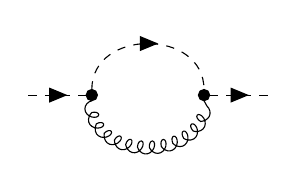
\begin{tikzpicture}[baseline=(current bounding box.center),scale=0.95,every node/.style={transform shape}]
\begin{feynman}
  \vertex (l) at (-0.85,0);
  \vertex [dot] (a) at (0,0) {};
  \vertex [dot] (b) at (1.5,0) {};
  \vertex (r) at (2.35,0);
  \diagram*{
    (l) -- [charged scalar] (a),
    (a) -- [charged scalar, half left, looseness=1.4] (b),
    (a) -- [gluon, half right, looseness=1.4] (b),
    (b) -- [charged scalar] (r),
  };
\end{feynman}
\end{tikzpicture}
&
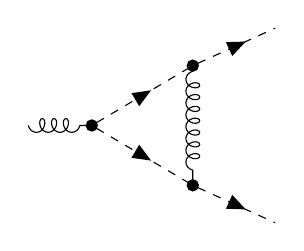
\begin{tikzpicture}[baseline=(current bounding box.center),scale=0.95,every node/.style={transform shape}]
\begin{feynman}
  \vertex (l) at (-0.85,0);
  \vertex [dot] (a) at (0,0) {};
  \vertex [dot] (b) at (1.35,0.80) {};
  \vertex [dot] (c) at (1.35,-0.80) {};
  \vertex (r1) at (2.45,1.30);
  \vertex (r2) at (2.45,-1.30);
  \diagram*{
    (l) -- [gluon] (a),
    (a) -- [charged scalar] (b),
    (a) -- [charged scalar] (c),
    (b) -- [gluon] (c),
    (b) -- [charged scalar] (r1),
    (c) -- [charged scalar] (r2),
  };
\end{feynman}
\end{tikzpicture}
&
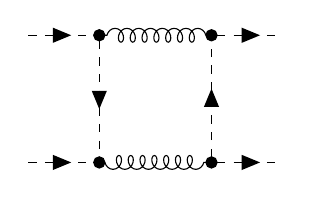
\begin{tikzpicture}[baseline=(current bounding box.center),scale=0.95,every node/.style={transform shape}]
\begin{feynman}
  \vertex (l1) at (-0.95,0.85);
  \vertex (l2) at (-0.95,-0.85);
  \vertex [dot] (a) at (0,0.85) {};
  \vertex [dot] (b) at (0,-0.85) {};
  \vertex [dot] (c) at (1.5,-0.85) {};
  \vertex [dot] (d) at (1.5,0.85) {};
  \vertex (r1) at (2.45,0.85);
  \vertex (r2) at (2.45,-0.85);
  \diagram*{
    (l1) -- [charged scalar] (a),
    (l2) -- [charged scalar] (b),
    (a) -- [charged scalar] (b),
    (b) -- [gluon] (c),
    (c) -- [charged scalar] (d),
    (d) -- [gluon] (a),
    (d) -- [charged scalar] (r1),
    (c) -- [charged scalar] (r2),
  };
\end{feynman}
\end{tikzpicture}
\\[1mm]
\footnotesize (a) bubble & \footnotesize (b) triangle & \footnotesize (c) box
\end{tabular}
\caption{Representative topologies of the massive master integrals. Solid
(charged-scalar) lines carry the mass $m$, coiled lines are massless gluons.
The full basis comprises the bubbles, one- and two-mass triangles and the one-
and two-mass boxes listed in Eqs.~\eqref{eq:basis-ab}--\eqref{eq:basis-nab}; each is
generated once
with $(s,t,u,m_i^2,m_k^2)$ as runtime parameters and compiled to a library.
Unlike their massless counterparts, Eqs.~\eqref{eq:I2}--\eqref{eq:I41m}, they
have no closed form in general.}
\label{fig:masters}
\end{figure}

While the massive triangles and boxes are evaluated numerically, the tadpole and
all massive bubbles are known in closed form to all orders in $\eps$, and
these expressions are part of the numerical framework (they replace the
sector-decomposed evaluation wherever they apply). In the bare normalisation
$\Gamma(\eps)\int(\text{Symanzik})^{-\eps}$ used by the code they read
\begin{align}
  A_0(m^2)&=\Gamma(\eps-1)\,(m^2)^{1-\eps}
   \;=\;-\frac{\Gamma(\eps)\,(m^2)^{1-\eps}}{1-\eps}\;,
  \label{eq:A0-closed}\\[1mm]
  \Bz{p^2}{0,m^2}&=\frac{\Gamma(\eps)\,(m^2-p^2)^{-\eps}}{1-\eps}\;
   {}_2F_1\!\left(\eps,\,1-\eps;\,2-\eps;\,\frac{-p^2}{m^2-p^2}\right),
  \label{eq:B0zm-closed}\\[1mm]
  \Bz{m^2}{0,m^2}&=\frac{\Gamma(\eps)\,(m^2)^{-\eps}}{1-2\eps}\;,
  \label{eq:B0os-closed}\\[1mm]
  \Bz{p^2}{m^2,m^2}&=\Gamma(\eps)\,(m^2)^{-\eps}
   \left(1-\frac{z}{4}\right)^{\!-\eps}
   {}_2F_1\!\left(\eps,\,\tfrac12;\,\tfrac32;\,\frac{-z}{4-z}\right),
   \qquad z=\frac{p^2}{m^2}\;.
  \label{eq:B0mm-closed}
\end{align}
Equation~\eqref{eq:B0os-closed} is the on-shell case of
Eq.~\eqref{eq:B0zm-closed}, where the ${}_2F_1$ form has a threshold pole and the
Feynman-parameter integral instead collapses to
$\int_0^1[m^2(1-x)^2]^{-\eps}=1/(1-2\eps)$. Every one of these closed forms was
verified against the sector-decomposed evaluation to $16$ digits at each order in
$\eps$ through $\eps^{3}$, at multiple Euclidean points; conversely they validate
the numerical machinery on the subset of masters where an exact answer exists.
The genuinely numerical content of the calculation is therefore confined to the
triangles and boxes.

A useful check follows immediately. The colour- and polarisation-summed
 {tree} squared amplitude of the scalar dipole is, in the singlet projection,
\begin{equation}
  \big|\mathcal{M}^{(0)}_{\tilde q}\big|^{2}
  =\frac{-16\,\Gram}{3\,(m^2-t)^2\,(m^2-u)^2}\;,
  \label{eq:tree-gram}
\end{equation}
i.e.\ the tree squared amplitude is itself proportional to the very Gram
determinant that controls the denominators of the one-loop reduction. Note that
$\Gram<0$ in the physical region, so Eq.~\eqref{eq:tree-gram} is positive there;
at the Euclidean points used for validation ($s,t,u<0$) the kinematics are not
realisable by real momenta and Eq.~\eqref{eq:tree-gram} is an analytic
continuation which may take either sign. We have checked
Eq.~\eqref{eq:tree-gram} numerically at physical soft configurations, where it
gives $500.0$ and $517.2$ at the two dipole invariants of Table~\ref{tab:bcm}.

Throughout, the reduction produces the Gram-type determinant
\begin{equation}
  \Gram = 4m^6-m^4\big(s+4t+4u\big)+m^2\big(t+u\big)\big(s+t+u\big)-s\,t\,u\;,
  \label{eq:gram}
\end{equation}
which together with $(m^2-t)$ and $(2m^2-t-u)$ exhausts the denominators of all
reduction coefficients; explicit expressions are given in
App.~\ref{app:coefficients}.

%=====================================================================
\section{Numerical evaluation}
\label{sec:numerics}
%=====================================================================
The masters are evaluated by sector decomposition with
\textsc{pySecDec}~\cite{pySecDec}. Each master is generated once with the
invariants $(s,t,u)$ and the masses $(m_i^2,m_k^2)$ declared as  {real
runtime parameters} and compiled to a shared library. A phase-space point is then
a single quasi-Monte-Carlo call into the compiled library. The dominant cost is
the one-time compilation, a few minutes for the full basis; each subsequent point
costs $\mathcal{O}(0.1)\,$s per master, i.e.\ sub-second per phase-space point.
This is what makes the method usable inside a fully differential Monte-Carlo
integration, and it is the virtual-side analogue of the numerical assembly of the
real-emission integrals in Ref.~\cite{Czakon:stripper}.

The libraries are built with contour deformation, so the same compiled basis is
used unchanged at Euclidean and at physical kinematics; in the physical region the
masters acquire the expected absorptive parts. This is essential for the soft
comparison of Sec.~\ref{sec:bcm}, which is intrinsically Minkowskian.

The masters are returned in the bare convention; the amplitude convention is
reached by the loop measure factor $i$ together with the global factor
\begin{equation}
  \frac{16\pi^2}{i}\left(\frac{e^{\gamma_E}}{4\pi}\right)^{\!\eps},
  \label{eq:msbarfac}
\end{equation}
so that the result is the bare $\msbar$ amplitude as a Laurent series in $\eps$
through $\eps^{3}$.

%=====================================================================
\section{Validation}
\label{sec:validation}
%=====================================================================

\subsection{Independent evaluation of every master (AMFlow)}
Every master integral was recomputed with the auxiliary-mass-flow
method~\cite{AMFlow}, which is algorithmically unrelated to sector decomposition:
it solves differential equations in an auxiliary mass, with IBP reduction
supplied by \textsc{Kira}. At a random Euclidean point the two evaluations agree
to the precision of the quasi-Monte-Carlo integration,
Table~\ref{tab:amflow}. The residual differences at $\eps^{3}$ reflect the
sector-decomposition uncertainty at high orders in $\eps$, not a disagreement:
AMFlow is the $20$-digit reference.

\begin{table}[t]
\centering
\caption{Maximum $|\,\text{AMFlow}-\textsc{pySecDec}\,|$ over
$\eps^{-2}\dots\eps^{3}$, at a random Euclidean point
($s=-3$, $t=-5$, $u=-2$; one-mass $m^2=1$; two-mass $m_i^2=1$, $m_k^2=2$).}
\label{tab:amflow}
\begin{tabular}{lcc}
\toprule
 & equal-mass & two-mass \\
\midrule
bubbles / triangles      & $10^{-9}\!-\!10^{-16}$ & $10^{-10}\!-\!10^{-15}$\\
boxes (worst, $\eps^3$)  & $8\times10^{-7}$       & $6.1\times10^{-7}$\\
\bottomrule
\end{tabular}
\end{table}

\subsection{Massless limit}
Taking $m\to0$ in the assembled abelian amplitude reproduces the massless result
of Ref.~\cite{Campbell:2025} order by order through $\eps^{3}$, at several
Euclidean points including fully asymmetric ones (ratio $=1$ to ten digits). The
$m_k\to m_i$ limit of the two-mass amplitude reproduces the one-mass amplitude to
quasi-Monte-Carlo precision.

The non-abelian sector admits a sharper test, because its massless limit is known
in closed form. Dividing the $m\to0$ limit of our massive non-abelian radiator by
the unsubtracted massless combination $\mathcal{B}^{\rm(nab)}$ of
Eq.~\eqref{eq:Bnab} gives a ratio that is  {independent of the kinematics},
\begin{equation}
  \frac{\mathcal{M}^{\rm nab}_{m\to0}}{\mathcal{B}^{\rm(nab)}}
  =-16\pi^2 i\,\big(1+0.5675\,\eps+\dots\big)\;,
  \label{eq:nabratio}
\end{equation}
identical at four independent Euclidean points to $\sim\!18$ digits, with the
leading coefficient reproducing the expected normalisation $-16\pi^2 i$ exactly.
Because the ratio is kinematics independent while the individual integrals are
not, this validates the non-abelian reduction coefficients, not merely the master
integrals. We stress that the comparison is against $\mathcal{B}^{\rm(nab)}$ and
not against $I_4^{\rm(nab)}$: the two differ by the counterterm bracket
\eqref{eq:BminusI4}, and using the latter would produce a kinematics-dependent
ratio.

\subsection{Gauge invariance}
\label{sec:ward}
The radiator satisfies the Ward identity symbolically. Writing the amplitude as
$\mathcal{M}^\mu\eps^*_\mu(q)=A\,(p_i\!\cdot\!\eps^*)+C\,(p_k\!\cdot\!\eps^*)$,
transversality of the emitted gluon requires
\begin{equation}
  \frac{t-m^2}{2}\,A+\frac{u-m^2}{2}\,C=0\;,
  \label{eq:ward-check}
\end{equation}
which is the statement that the radiator carries the dipole structure
$p_i^\mu/(t-m^2)-p_k^\mu/(u-m^2)$. We have verified Eq.~\eqref{eq:ward-check}
 {as an exact algebraic identity} in the reduced amplitude: the combination
vanishes coefficient by coefficient on the master integrals, with the masses and
invariants kept symbolic, so it holds at every kinematic point rather than
numerically at sampled ones. This is a third, independent check, complementary to
the two above: the massless limit and the soft limit test the amplitude against
external results, whereas gauge invariance is an internal consistency of the full
reduction, sensitive to the relative normalisation of every diagram and every
reduction coefficient at once.

\subsection{The soft limit against the massive one-loop soft current}
\label{sec:bcm}
The strongest external check available is the soft limit. The one-loop soft
current for massive emitters is known~\cite{BCM}; it is purely non-abelian,
\begin{equation}
  J^{\mu(1)}_a(q)=i f_{abc}\sum_{i\neq j}\Top{i}^b\Top{j}^c
    \left(e_i^\mu-e_j^\mu\right)g^{(1)}_{ij}\;,\qquad
  e_i^\mu=\frac{p_i^\mu}{p_i\!\cdot\!q}\;,
  \label{eq:softcurrent}
\end{equation}
and for the configuration relevant here, both emitters massive
(``Case~3'' of Ref.~\cite{BCM}), the normalised function is defined with an
explicit kinematic prefactor,
\begin{equation}
  g^{(1)}_{ij}\Big|_{\rm Case\,3}=a_S^b
  \left(\frac{2\,p_ip_j\,\mu^2}{2\,p_iq\;2\,p_jq}\right)^{\!\eps}
  \sum_{n=-2}^{1}\eps^n\Big(R^{(n)}_{ij}+i\pi I^{(n)}_{ij}\Big)\;,
  \qquad R^{(-2)}_{ij}=-\tfrac12\;,
  \label{eq:gij}
\end{equation}
with $a_S^b=\alpha_s^b S_\eps/(2\pi)$. The prefactor is essential: the tabulated
coefficients $R^{(n)},I^{(n)}$ carry none of the dependence on the softness of
$q$, which resides entirely in $(2p_iq\,2p_jq)^{-\eps}$.

We map our invariants onto theirs by $p_i=p_i$, $p_j=p_k$, $q=q$, i.e.
\begin{equation}
  m_i^2=m_j^2=m^2\;,\qquad
  p_ip_j=\frac{s-2m^2}{2}\;,\qquad
  p_iq=\frac{t-m^2}{2}\;,\qquad
  p_jq=\frac{u-m^2}{2}\;,
  \label{eq:bcmmap}
\end{equation}
and construct genuinely soft,  {physical} configurations by fixing the two
massive emitters exactly on shell and scaling the emitted gluon as $q=w\,n$ with
$n$ light-like. Then $s$ is independent of $w$ while $t-m^2$ and $u-m^2$ vanish
linearly. Soft factorisation predicts, for the coefficient of $p_i\!\cdot\!\eps$,
\begin{equation}
  \mathcal{M}^{\rm nab}\Big|_{\rm soft}=N(\eps)\,\frac{g^{(1)}_{ij}}{p_i\!\cdot\!q}\;,
  \label{eq:softpred}
\end{equation}
with $N(\eps)$ independent of the kinematics, so that
$\mathcal{M}^{\rm nab}\,(p_i\!\cdot\!q)/g^{(1)}_{ij}$ must be one and the same
Laurent series everywhere.

Table~\ref{tab:bcm} shows that it is, and does so in absolute terms rather than
only as a constant ratio: at $\eps^{-2}$ the BCM coefficient $R^{(-2)}_{ij}=-\tfrac12$
predicts
\begin{equation}
  \mathcal{M}^{\rm nab}\Big|_{\eps^{-2}}=\frac{32\pi^2\,i}{p_i\!\cdot\!q}\;,
  \label{eq:bcm-abs}
\end{equation}
with no freedom left once the single overall constant is fixed, and our numbers
reproduce this at every configuration to $11$--$13$ digits. Equivalently, the
$\eps^0$ coefficient of the ratio is
\begin{equation}
  \frac{\mathcal{M}^{\rm nab}\,(p_i\!\cdot\!q)}{g^{(1)}_{ij}}\bigg|_{\eps^0}
  =-631.6546817\,i=-64\pi^2 i\;,
  \label{eq:bcmresult}
\end{equation}
identical to ten significant figures at all eight configurations, spanning two
values of $s$ and a decade in softness. Equivalently, the double pole of the
massive non-abelian radiator obeys the exact eikonal scaling
$\mathcal{M}^{\rm nab}\big|_{\eps^{-2}}=32\pi^2 i/(p_i\!\cdot\!q)$, again to ten
digits and at both values of $s$. This is a genuine external validation: it tests
the massive amplitude at physical kinematics, in a region where every master
carries a nontrivial absorptive part, against a result obtained by completely
different means.

\begin{table}[htbp]
\centering
\caption{Direct numerical comparison of our massive non-abelian radiator with the
one-loop massive soft current of Ref.~\cite{BCM}, Case~3, at $m^2=1$. The two
massive emitters are held fixed and the gluon is scaled as $q=w\,n$. Column three
is the $\eps^{-2}$ coefficient of our amplitude, computed from the compiled master
libraries at physical kinematics; column four is the BCM prediction
$32\pi^2/(p_i\!\cdot\!q)$, which follows from $R^{(-2)}_{ij}=-\tfrac12$ together
with the single normalisation constant $N_0=-64\pi^2 i$. Both are purely
imaginary; the tabulated entries are $\mathrm{Im}$. One constant is fixed once and
for all  --  and it is independently $4\times$ the massless normalisation
$-16\pi^2 i$ found against Ref.~\cite{Campbell:2025}  --  after which the remaining
eight entries are absolute predictions, reproduced to $11$--$13$ significant
figures. The residual deviations are at the level of the quasi-Monte-Carlo
uncertainty of the masters.}
\label{tab:bcm}
\begin{tabular}{ccccc}
\toprule
$s$ & $w$ & ours: $\mathrm{Im}\,\mathcal{M}^{\rm nab}\big|_{\eps^{-2}}$
    & BCM: $32\pi^2/(p_i\!\cdot\!q)$ & ratio\\
\midrule
$20$ & $0.10$ & $2555.0968602$ & $2555.0968602$ & $1.000000000000$\\
$20$ & $0.05$ & $5110.1937205$ & $5110.1937205$ & $0.999999999999$\\
$20$ & $0.02$ & $12775.4843010$ & $12775.4843012$ & $0.999999999985$\\
$20$ & $0.01$ & $25550.9686024$ & $25550.9686024$ & $1.000000000000$\\
$40$ & $0.10$ & $777.4636971$ & $777.4636971$ & $1.000000000000$\\
$40$ & $0.05$ & $1554.9273942$ & $1554.9273942$ & $1.000000000000$\\
$40$ & $0.02$ & $3887.3184855$ & $3887.3184855$ & $0.999999999999$\\
$40$ & $0.01$ & $7774.6369706$ & $7774.6369711$ & $0.999999999935$\\
\bottomrule
\end{tabular}
\end{table}

%=====================================================================
\section{Absence of collinear sectorization for massive partons}
\label{sec:nosector}
%=====================================================================
The organising principle of Ref.~\cite{Campbell:2025} is that soft and collinear
limits do not commute, so that the splitting functions contain overlapping
soft--collinear singularities. In existing NNLO subtraction schemes that overlap
is disentangled by phase-space sectorization.

For massive partons the situation simplifies, but in a way that requires care.
The mass regulates the collinear region: a propagator $1/(p^2-m^2)$ produces no
collinear $1/\eps$ pole as $p^2\to m^2$. We find that this screening acts
 {entirely on the abelian sector}. Decomposing the complete radiator by
colour structure we obtain, numerically,
\begin{equation}
  \mathcal{M}^{(1)}\Big|^{\rm abelian}_{\eps^{-2}}=0\;,
  \qquad
  \mathcal{M}^{(1)}\Big|^{\rm non\text{-}abelian}_{\eps^{-2}}\neq0\;,
  \label{eq:noeps2}
\end{equation}
the latter purely imaginary, as required by the $if^{abc}$ colour structure. The
abelian double pole, which in the massless theory arises from the  {overlap}
of the soft and collinear regions, is switched off by the mass. What survives is
the non-abelian double pole of the one-loop soft current, which is universal and
already known in closed form  --  and which Sec.~\ref{sec:bcm} shows we reproduce
exactly.

This distinction is the essential point. Sectorization exists to disentangle the
soft--collinear  {overlap}; it is not needed for a pure soft singularity.
Since the massive amplitude retains only the latter, the overlap is absent and no
phase-space sectorization is required.

Both features are corroborated by Ref.~\cite{BCM}. First, the one-loop massive
soft current \eqref{eq:softcurrent} is purely non-abelian, with no abelian
contribution  --  precisely why the double pole we find is confined to the
non-abelian structure and is purely imaginary. Second, for both emitters massive,
Ref.~\cite{BCM} states explicitly that collinear singularities are regularised
and do not lead to poles in $\eps$, in agreement with Table~\ref{tab:collinear}.

\subsection{Numerical demonstration}
The statement can be exhibited directly. We fix $s=-3$, $u=-2$ and drive the
amplitude into the collinear region $t\to0$ at two values of the mass.
Table~\ref{tab:collinear} lists the $\eps^{-1}$ coefficient of the abelian
amplitude together with its increment between successive points. A genuine
collinear singularity produces a  {constant} increment per fixed ratio of
$|t|$, i.e.\ logarithmic growth; a mass-regulated amplitude approaches a finite
limit, so the increments must die away.

\begin{table}[t]
\centering
\caption{Collinear scan of the abelian massive amplitude at $s=-3$, $u=-2$. For
$m^2=1$ the increments collapse geometrically and the coefficient converges to a
finite limit $\approx2.94$. For $m^2=0.01$, with $|t|\gtrsim m^2$ over most of
the range, the increments instead approach a constant  --  the signature of
logarithmic collinear growth  --  and the coefficient grows by nearly two orders
of magnitude. The mass cuts the collinear region off at $|t|\sim m^2$.}
\label{tab:collinear}
\begin{tabular}{lcccc}
\toprule
 & \multicolumn{2}{c}{$m^2=1$} & \multicolumn{2}{c}{$m^2=0.01$}\\
\cmidrule(lr){2-3}\cmidrule(lr){4-5}
$t$ & $\eps^{-1}$ & $\Delta$ & $\eps^{-1}$ & $\Delta$\\
\midrule
$-1$      & $1.4730$ &  --      & $8.199$ &  -- \\
$-0.3$    & $2.2662$ & $0.793$ & $26.71$ & $18.5$\\
$-0.1$    & $2.6782$ & $0.412$ & $75.28$ & $48.6$\\
$-0.03$   & $2.8602$ & $0.182$ & $207.0$ & $131.7$\\
$-0.01$   & $2.9169$ & $0.057$ & $414.0$ & $207.0$\\
$-0.003$  & $2.9372$ & $0.020$ & $636.9$ & $222.9$\\
\bottomrule
\end{tabular}
\end{table}

The double pole vanishes identically throughout the scan, so the finite $t\to0$
limit at $m^2=1$ is not an artefact of a cancellation between orders: the abelian
amplitude is simply free of collinear singularities once the mass is switched on.
Table~\ref{tab:poles} collects the leading Laurent coefficients.

\begin{table}[t]
\centering
\caption{Leading Laurent coefficients of the assembled amplitude. Upper block:
the abelian, $p_i$-projected amplitude, whose double pole vanishes for $m\neq0$.
Lower block: the $\eps^{-2}$ coefficient of the complete radiator at
$(s,t,u)=(-3,-5,-2)$, $m^2=1$, separated by colour structure. Only the
non-abelian structure retains a double pole, and it is purely imaginary.}
\label{tab:poles}
\begin{tabular}{lccc}
\toprule
point & $\eps^{-2}$ & $\eps^{-1}$ & $\eps^{0}$\\
\midrule
$(-1,-1,-1)$, $m^2=1$              & $0$ & $1.194$ & $-1.766$\\
$(-2,-3,-1)$, $m^2=1$              & $0$ & $0.674$ & $-0.743$\\
$(-2,-3,-1)$, $m_i^2=1$, $m_k^2=2$ & $0$ & $0.640$ & $-1.029$\\
\midrule
\multicolumn{4}{l}{by colour structure at $(-3,-5,-2)$, $m^2=1$:}\\
\quad abelian     & $0$          & $0.4910$    & $-0.6169$\\
\quad non-abelian & $-105.28\,i$ & $507.08\,i$ & $-708.86\,i$\\
\bottomrule
\end{tabular}
\end{table}

\noindent
The two colour structures are stripped by different prefactors, so their relative
normalisation is not fixed here. The statement that matters, and which is
normalisation independent, is that the abelian double pole  {vanishes} while
the non-abelian one does not.

Since the scalar dipole radiator captures precisely the soft structure, and the
soft structure is now the  {entire} singular structure, the massive one-loop
splitting amplitude  {is} its scalar dipole radiator up to a finite,
spin-dependent remainder. The double-real and real--virtual massive contributions
carry soft-only singularities and can be subtracted with a single soft
counterterm, implemented as an additional Monte-Carlo channel sampled only to the
precision the observable requires, exactly as in the fully numerical treatment of
Ref.~\cite{Czakon:stripper}. This is the sense in which the massive NNLO
calculation is structurally simpler than its massless counterpart.

%=====================================================================
\section{The scalar radiator is the complete heavy-quark ingredient}
\label{sec:splitting}
%=====================================================================
In the decomposition of Ref.~\cite{Campbell:2025} the quark--gluon vertex is
written as a scalar piece, a magnetic piece and a term proportional to the
equations of motion,
\begin{equation}
  \bar u(p')\gamma^\mu u(p)\;\longrightarrow\;
  \underbrace{S^\mu(p,q)}_{\text{scalar radiator}}
  \;+\;\underbrace{\frac{i\,\sigma^{\mu\nu}q_\nu}{(p+q)^2-m^2}}_{\text{magnetic}}
  \;+\;\text{(EOM)}\;,
  \label{eq:vertex-decomposition}
\end{equation}
so that a massive quark splitting amplitude is the scalar dipole radiator plus a
magnetic (spin) remainder. The decisive point for a heavy quark is where these two
pieces are singular. The scalar radiator carries the soft singularity,
which is universal and mass-independent. The magnetic remainder is singular only in
the genuine collinear limit; as Sec.~\ref{sec:nosector} shows, that
limit is regulated by the mass: for $m\neq0$ the propagator $1/((p+q)^2-m^2)$ in
Eq.~\eqref{eq:vertex-decomposition} produces no collinear pole. The magnetic
remainder is therefore finite for a massive quark.

The consequence, already anticipated by Czakon in the context of massive NNLO
subtraction, is that the scalar radiator is the complete ingredient. A
subtraction term must reproduce the singular structure of the amplitude; since the
massive amplitude's entire singular structure is the soft one, and that is exactly
the scalar dipole radiator, no further piece is required. There is no separate
collinear (spin) counterterm to assemble, precisely because there is no collinear
singularity to subtract. This is the same statement as the absence of
sectorization: the soft--collinear overlap that a spin remainder would be needed to
organise is simply not present once the mass is switched on.

We stress that this is special to the heavy-quark (massive) case. For a massless
quark the magnetic remainder is collinear-divergent and does contribute to the
splitting function~\cite{Campbell:2025}; its finite massive counterpart is a
genuine but power-suppressed, subtraction-irrelevant quantity. The scalar radiator
computed and validated above is thus not one of two ingredients but the whole of
what a fully numerical massive NNLO subtraction needs.

%=====================================================================
\section{Conclusions}
\label{sec:conclusions}
%=====================================================================
We have computed the massive one-loop scalar dipole radiator, the massive
analogue of the box-type contributions of Ref.~\cite{Campbell:2025}, fully
numerically. The master integrals are compiled once with the kinematics and
masses as runtime parameters and evaluated in sub-second time per phase-space
point, with contour deformation so that the same basis serves Euclidean and
physical kinematics alike.

The calculation is validated three ways: every master against auxiliary-mass
flow; the assembled amplitude against the closed-form massless expressions in the
$m\to0$ limit, where the non-abelian ratio is kinematics independent to $18$
digits; and the soft limit against the one-loop massive soft current of
Ref.~\cite{BCM}, where the double pole is reproduced with the single
kinematics-independent normalisation $-64\pi^2 i$ at eight physical
configurations. Along the way we clarified that a direct diagrammatic computation
returns the unsubtracted combination \eqref{eq:Bnab}, which differs from the
quoted $I_4^{\rm(nab)}$ by exactly the factorization counterterm.

The mass screens the collinear singularity, so the radiator is the complete
singular structure and the massive NNLO subtraction needs no sectorization. The
same fact makes the radiator the complete heavy-quark ingredient: the
magnetic (spin) remainder is singular only in the collinear limit, which the mass
regulates, so it is finite and subtraction-irrelevant, and there is no further
splitting-function piece to assemble (Sec.~\ref{sec:splitting}). Together with the
fully numerical assembly of the real-emission integrals, this shows that a
FONLL-matched, fully numerical NNLO calculation of heavy-quark production for
FCC-ee rests on an ingredient that is now in hand.

\acknowledgments
The author thanks S.~H\"oche, M.~Knobbe and the authors of
Ref.~\cite{Campbell:2025} for discussions.


\appendix
%=====================================================================
\section{Reduced amplitudes in terms of the master integrals}
\label{app:coefficients}
%=====================================================================
We give the complete reduction of the massive radiator, so that the result can be
reproduced, or the master integrals recomputed, independently. Everything below
refers to the coefficient of $p_i\!\cdot\!\eps^*(q)$; the $p_k$ projection follows
by $i\leftrightarrow k$, $t\leftrightarrow u$. The Gram-type determinant $\Gram$
is defined in Eq.~\eqref{eq:gram}. The reduction leaves  {no} rational
remainder: each amplitude is exactly a linear combination of the masters listed in
Eqs.~\eqref{eq:basis-ab}--\eqref{eq:basis-nab}.

Throughout, $N\equiv N_c$, and the coefficients are pure rational functions of
$(s,t,u,m^2)$; they are given in factored form, with the Gram determinant $\Gram$
of Eq.~\eqref{eq:gram} appearing in the box-coefficient denominators.

\subsection{Non-abelian radiator}
\label{app:nab}
Stripped of the colour and coupling prefactor
$g_s^3 f^{abc}\,T^b_{c_ic_j}T^c_{c_kc_l}/(16\pi^2)$, the non-abelian radiator is
\begin{equation}
  \mathcal{M}^{\rm nab}=\sum_{j}\,c^{\rm nab}_j\;I_j\;,
  \label{eq:nab-reduction}
\end{equation}
with $I_j$ running over the $14$ masters of Eq.~\eqref{eq:basis-nab} and the
coefficients $c^{\rm nab}_j$
\begin{align*}
\scriptsize
\input{app_nab.tex}
\end{align*}

\subsection{Abelian radiator}
\label{app:ab}
The abelian radiator is not a single colour structure. Expanded in the four
colour monomials
\begin{equation}
\begin{aligned}
  \mathcal{C}_1&=\delta_{c_kc_l}\,T^a_{c_ic_j}\;,&\qquad
  \mathcal{C}_2&=\delta_{c_jc_k}\,T^a_{c_ic_l}\;,\\
  \mathcal{C}_3&=\delta_{c_ic_l}\,T^a_{c_kc_j}\;,&\qquad
  \mathcal{C}_4&=\delta_{c_ic_j}\,T^a_{c_kc_l}\;,
\end{aligned}
\label{eq:colour-monomials}
\end{equation}
it reads, stripped of $g_s^3/(16\pi^2)$,
\begin{equation}
  \mathcal{M}^{\rm ab}=\sum_{r=1}^{4}\mathcal{C}_r\sum_j\,c^{(r)}_j\,I_j\;,
  \label{eq:ab-reduction}
\end{equation}
with the $I_j$ drawn from Eq.~\eqref{eq:basis-ab}. The coefficients $c^{(r)}_j$
are, for $\mathcal{C}_1$,
\begin{align*}
\scriptsize
\Bz{m^2}{0,m^2} &:\; \dfrac{2 Ii }{N \left(m^2-t\right)} \\[2mm]
\Bz{s}{m^2,m^2} &:\; \dfrac{-Ii }{N \left(2 m^2-t-u\right)} \\[2mm]
\Bz{t}{0,m^2} &:\; 0i  \\[2mm]
\Bz{Q^2}{m^2,m^2} &:\; \dfrac{-Ii \left(m^2-u\right)}{N \left(m^2-t\right) \left(2 m^2-t-u\right)} \\[2mm]
\Cz{0,m^2,t}{m^2,m^2,0} &:\; \dfrac{-Ii \left(2 m^2-s\right)\left(m^2-t\right)\left(m^2-u\right)}{\Gram N} \\[2mm]
\Cz{0,s,Q^2}{m^2,m^2,m^2} &:\; \dfrac{Ii \left(2 m^2-s\right)\left(m^2-u\right)\left(2 m^2-t-u\right)}{\Gram N} \\[2mm]
\Cz{m^2,m^2,s}{m^2,0,m^2} &:\; \dfrac{i \left(2 m^2-s\right)\big(\begin{aligned}[t]&4 m^4 - m^2 s - 2 m^2 t - 2 m^2 u + s u \big)\end{aligned}}{\Gram N} \\[2mm]
\Cz{m^2,t,Q^2}{m^2,0,m^2} &:\; \dfrac{i \left(m^2-u\right)\big(\begin{aligned}[t]&14 m^6 - 7 m^4 s + m^2 s^2 - 10 m^4 t + 5 m^2 s t \\
  &\qquad - s^2 t + 2 m^2 t^2 - 10 m^4 u + 3 m^2 s u + 2 m^2 t u \\
  &\qquad - s t u + 2 m^2 u^2 \big)\end{aligned}}{\Gram N \left(m^2-t\right)} \\[2mm]
\Dzz{b} &:\; \dfrac{i \left(2 m^2-s\right)\left(m^2-u\right)\big(\begin{aligned}[t]&4 m^4 - m^2 s - 2 m^2 t + s t - 2 m^2 u \big)\end{aligned}}{\Gram N}
\end{align*}
for $\mathcal{C}_2$,
\begin{align*}
\scriptsize
\input{app_ab2.tex}
\end{align*}
for $\mathcal{C}_3$,
\begin{align*}
\scriptsize
\input{app_ab3.tex}
\end{align*}
and for $\mathcal{C}_4$,
\begin{align*}
\scriptsize
\Bz{m^2}{0,m^2} &:\; 0i  \\[2mm]
\Bz{s}{m^2,m^2} &:\; \dfrac{-Ii }{N \left(2 m^2-t-u\right)} \\[2mm]
\Bz{u}{0,m^2} &:\; 0i  \\[2mm]
\Bz{Q^2}{m^2,m^2} &:\; \dfrac{Ii }{N \left(2 m^2-t-u\right)} \\[2mm]
\Cz{0,m^2,u}{m^2,m^2,0} &:\; \dfrac{Ii \left(2 m^2-s\right)\left(m^2-u\right)^{2}}{\Gram N} \\[2mm]
\Cz{0,s,Q^2}{m^2,m^2,m^2} &:\; \dfrac{-Ii \left(2 m^2-s\right)\left(m^2-u\right)\left(2 m^2-t-u\right)}{\Gram N} \\[2mm]
\Cz{m^2,m^2,s}{m^2,0,m^2} &:\; \dfrac{i \left(2 m^2-s\right)\big(\begin{aligned}[t]&4 m^4 - m^2 s - 2 m^2 t - 2 m^2 u + s u \big)\end{aligned}}{\Gram N} \\[2mm]
\Cz{m^2,u,Q^2}{m^2,0,m^2} &:\; \dfrac{i \big(\begin{aligned}[t]&14 m^6 - 7 m^4 s + m^2 s^2 - 10 m^4 t + 3 m^2 s t \\
  &\qquad + 2 m^2 t^2 - 10 m^4 u + 5 m^2 s u - s^2 u + 2 m^2 t u \\
  &\qquad - s t u + 2 m^2 u^2 \big)\end{aligned}}{\Gram N} \\[2mm]
\Dzz{a} &:\; \dfrac{i \left(2 m^2-s\right)\left(m^2-u\right)\big(\begin{aligned}[t]&4 m^4 - m^2 s - 2 m^2 t - 2 m^2 u + s u \big)\end{aligned}}{\Gram N}
\end{align*}
The pairs $(\mathcal{C}_1,\mathcal{C}_4)$ and $(\mathcal{C}_2,\mathcal{C}_3)$ are
related by the $i\leftrightarrow k$, $t\leftrightarrow u$ exchange, which provides
an internal check on the reduction.

\begin{thebibliography}{9}

\bibitem{Campbell:2025}
J.~M.~Campbell, S.~H\"oche, M.~Knobbe, C.~T.~Preusz and D.~Reichelt,
``QCD splitting functions beyond kinematical limits,''
arXiv:2505.10408 [hep-ph].

\bibitem{pySecDec}
S.~Borowka, G.~Heinrich, S.~Jahn, S.~P.~Jones, M.~Kerner, J.~Schlenk and
T.~Zirke, ``pySecDec: a toolbox for the numerical evaluation of multi-scale
integrals,'' Comput.\ Phys.\ Commun.\ \textbf{222} (2018) 313,
arXiv:1703.09692 [hep-ph].

\bibitem{AMFlow}
X.~Liu and Y.-Q.~Ma, ``AMFlow: A Mathematica package for Feynman integrals
computation via auxiliary mass flow,''
Comput.\ Phys.\ Commun.\ \textbf{283} (2023) 108565,
arXiv:2201.11669 [hep-ph].

\bibitem{BCM}
I.~Bierenbaum, M.~Czakon and A.~Mitov, ``The singular behavior of one-loop
massive QCD amplitudes with one external soft gluon,''
Nucl.\ Phys.\ B \textbf{856} (2012) 228,
arXiv:1107.4384 [hep-ph].

\bibitem{BDK}
Z.~Bern, L.~J.~Dixon and D.~A.~Kosower, ``Dimensionally regulated pentagon
integrals,'' Nucl.\ Phys.\ B \textbf{412} (1994) 751, arXiv:hep-ph/9306240;
Z.~Bern, L.~J.~Dixon and D.~A.~Kosower, ``One-loop corrections to five-gluon
amplitudes,'' Phys.\ Rev.\ Lett.\ \textbf{70} (1993) 2677,
arXiv:hep-ph/9302280.

\bibitem{Kosower:1999rx}
D.~A.~Kosower, ``All-order collinear behavior in gauge theories,''
Nucl.\ Phys.\ B \textbf{552} (1999) 319, arXiv:hep-ph/9901201.

\bibitem{Catani:2000pi}
S.~Catani and M.~Grazzini, ``The soft-gluon current at one-loop order,''
Nucl.\ Phys.\ B \textbf{591} (2000) 435, arXiv:hep-ph/0007142.

\bibitem{Czakon:stripper}
M.~Czakon, ``A novel subtraction scheme for double-real radiation at NNLO,''
Phys.\ Lett.\ B \textbf{693} (2010) 259, arXiv:1005.0274 [hep-ph];
M.~Czakon and D.~Heymes, ``Four-dimensional formulation of the sector-improved
residue subtraction scheme,'' Nucl.\ Phys.\ B \textbf{890} (2014) 152,
arXiv:1408.2500 [hep-ph].

\end{thebibliography}

\end{document}
